






\documentclass[a4paper]{article}

\usepackage{amsmath,amssymb,amsfonts}
\usepackage{graphicx,float,subfig}
\usepackage{booktabs}
\usepackage{fullpage}
\usepackage[colorlinks]{hyperref}
\usepackage{pdflscape}

\usepackage[font=small,labelfont=bf]{caption}

\renewcommand{\abstractname}{Aim}

\title{Analysis of Gamma Ray Spectra from Reference Isotopes with Multi-Channel Analyzers}
\author{
    Oliver Kirkaptrick\footnote{s3725341@student.rmit.edu.au},
    Jackie Sholes\footnote{s3785864@student.rmit.edu.au},
    Anmolpreet Kaur Sodhi\footnote{s3838252@student.rmit.edu.au}
}


\begin{document}

\maketitle

\begin{abstract}
    In this experiment, we aim to to identify properties of obtained gamma ray spectra provided by known and unkown sampled. Additionally, using this information, we seek to use Full Width Half Maximum (FWHM) of the obtained spectra to estimate the resolution of detector hardware.
    % This study employs a Multi-Channel Analyzer to acquire gamma ray spectra of reference isotopes, aiming to explain the features observed in the spectra and determine the detector resolution as a function of energy. The output pulse from the detector is proportional to the energy of the gamma or X-ray that produced the interaction via the photoelectric process. Events resulting from the Compton effect produce a well-distributed low-energy area in the spectrum, as well as contributing to the full energy peak when the scattered photons undergo additional interactions. The pair production process may also contribute to the full energy peak if both the electron and positron's energy are deposited in the detector. The annihilation of the positron may produce a single or double escape peak.
\end{abstract}

\section{Relevant Theory}

Gamma rays entering the the detector (a Sodium Iodide scintillation detector) will produce electrons via photoelectr effect, compton effect, or pair production.

We can isolate these effects from one another via distributions of energies of the produced electrons. Compton effects should be observed across a wide range of low energy, low relative counts. A significantly large (relative to other effects) counts of higher energy electrons will produce a photopeak, indicating the photoelectric effect. These higher energies are a result of the gamma/x rays giving all their energies to the produced electrons. These photo peaks may also be contributed to by the production of pairs of electrons and positrons.

For a given incident gamma ray of energy $E_{\gamma}$, the energy due to scattering ($E_{\gamma}'$) can be given byx
\begin{equation}
    E_{\gamma}'=\frac{E_{\gamma}}{1+\left(1-\cos\theta\right)\left(\frac{E_{\gamma}}{m_{e}c^{2}}\right)},
\end{equation}
for a given scatter angle $\theta$. Here the mass energy $m_{e}c^{2}$ can be taken as 511 keV.

Inside the distribution of lower energy counts produced by the compton effect, we expect a smaller peak due to backscatter effects. The energies of the gamma rays contributing to this peak can be obtained by setting $\theta=180^{\circ}$.



\subsection{General Notes}

\begin{itemize}
    \item backscatter implies $\theta=180^{\circ}$
    \item At $E_{\gamma}\leq100\mathrm{\;keV}$, photo electric effect is dominant
    \item At $100\mathrm{\;keV}<E_{\gamma}\leq10000\mathrm{\;keV}$ compton scattering is dominant
    \item At $E_{\gamma}>10000\mathrm{\;keV}$, pair production is dominant
    \item 10V / 2048 mV(?) bins, so resolution is
\end{itemize}
\begin{equation}
    R=\frac{50\;\mathrm{mV}}{2048????}
\end{equation}
\begin{itemize}
    \item every channel number has an associated energy, Oscilloscope or MCB (???) associates bin number with energy
\end{itemize}

\section{Experiment Setup and Hardware}

For this experiment, the following hardware was used, in the configuration depicted in~\autoref{fig:hardware-config}:
\begin{itemize}
    \item NIM Bin and Power Supply
    \item NaI(Tl) Crystal and Phototube Assembly
    \item High Voltage Power Supply
    \item Preamplifier
    \item Amplifier
    \item Oscilloscope
    \item Multi Channel Analyser: Ortec 928 Multi Channel Buffer, USB dual Port Memory cable, PC with Maestro32 spectrum software.
    \item $^{137}\mathrm{Cs}$, $^{22}\mathrm{Na}$, and $^{60}\mathrm{Co}$ gamma sources
    \item gain is adjusted from 0.5, to bring max Oscilloscope reading to $\approx4$
    \item coarse gain is 100, fine is 0.571
    \item total gain is 57.1
\end{itemize}

\begin{figure}[H]
    \centering
    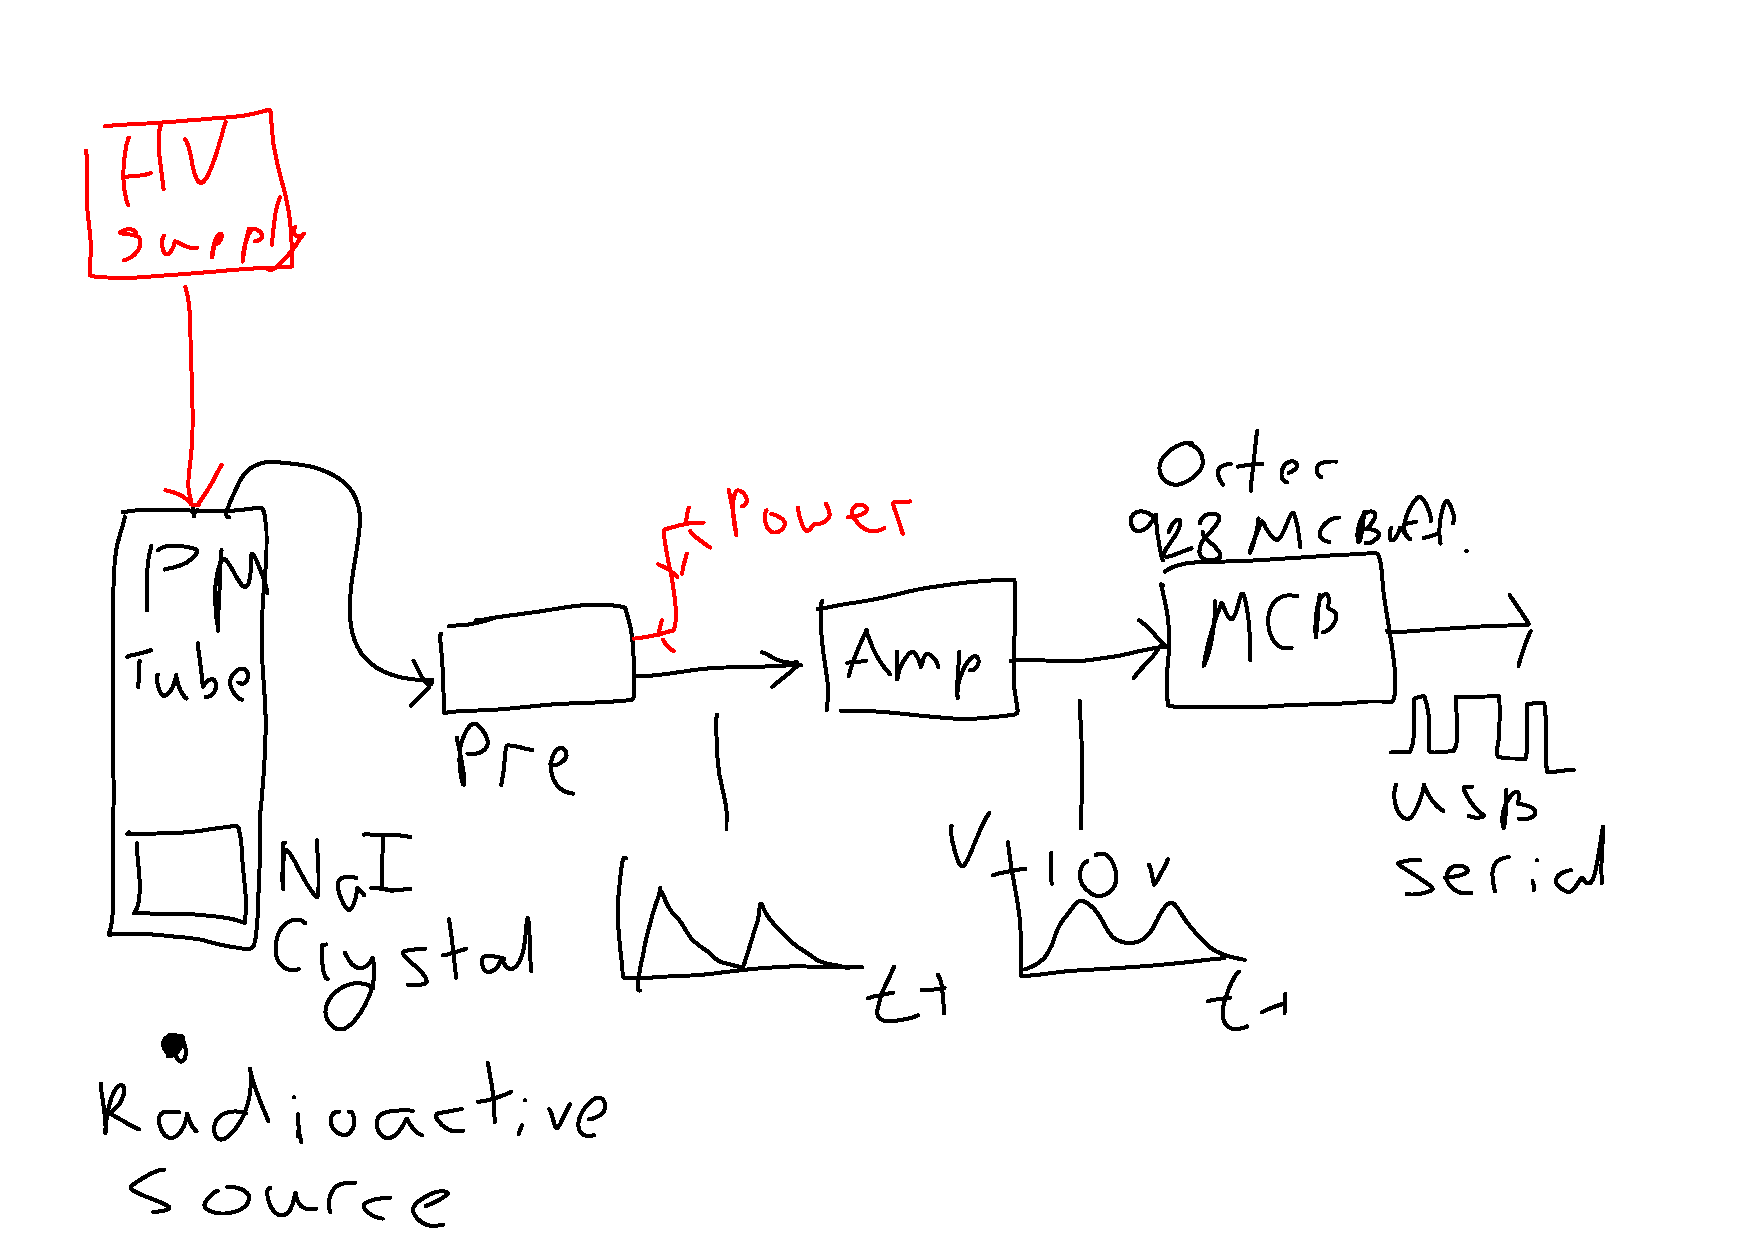
\includegraphics[width=0.6\textwidth]{figures/experiment-setup.pdf}
    \caption{Configuration of hardware for experiment. Raw signals originate at the Photo Multiplier Tube (PM Tube in figure), which is triggered by the radioactive source, which was placed approximately 2.5 cm in front of the PM Tube. These signals are fed into the Pre-Amplifier, (Pre Amp in figure), before passing into the amplifier. The signal has peaks at approximately 10 Volts after exiting the amplifier, where it is then fed into the Multi-Channel Buffer. Data from the Multi-Channel Buffer is analyzed on a computer via Spectrum32 software.}
    \label{fig:hardware-config}
\end{figure}

\subsection{Setup Procedures}

\begin{enumerate}
    \item HV connected to detector
    \item serial connected to pre amp
    \item signal out of detector connected to 572A input
    \item t bridge out of uni connected to Oscilloscope and 928 mcb adc in
    \item initial scale from Oscilloscope is 700 mV
    \item initial pulse width is 3.36 $\mu$s
\end{enumerate}

\section{Spectrum Analysis of $^{137}\mathrm{Cs}$, $^{22}\mathbf{Na}$, and $^{60}\mathrm{Co}$}
\subsection{Calibration}
\begin{itemize}
    \item initial height of photopeak was 1092 counts at live value of 10 seconds
    \item integration time increased to live value of 30 seconds
    \item 30 seconds produce 3107 counts
    \item ROI was set on 32 keV peak, and 662 keV peak
    \item 662 keV peak was identified as 662 keV, at bin 768.32, with FWHM of 43.84, library identified as cs 137
\end{itemize}

\subsection{Spectrum of $^{137}$Cs}
\begin{figure}[H]
    \centering
    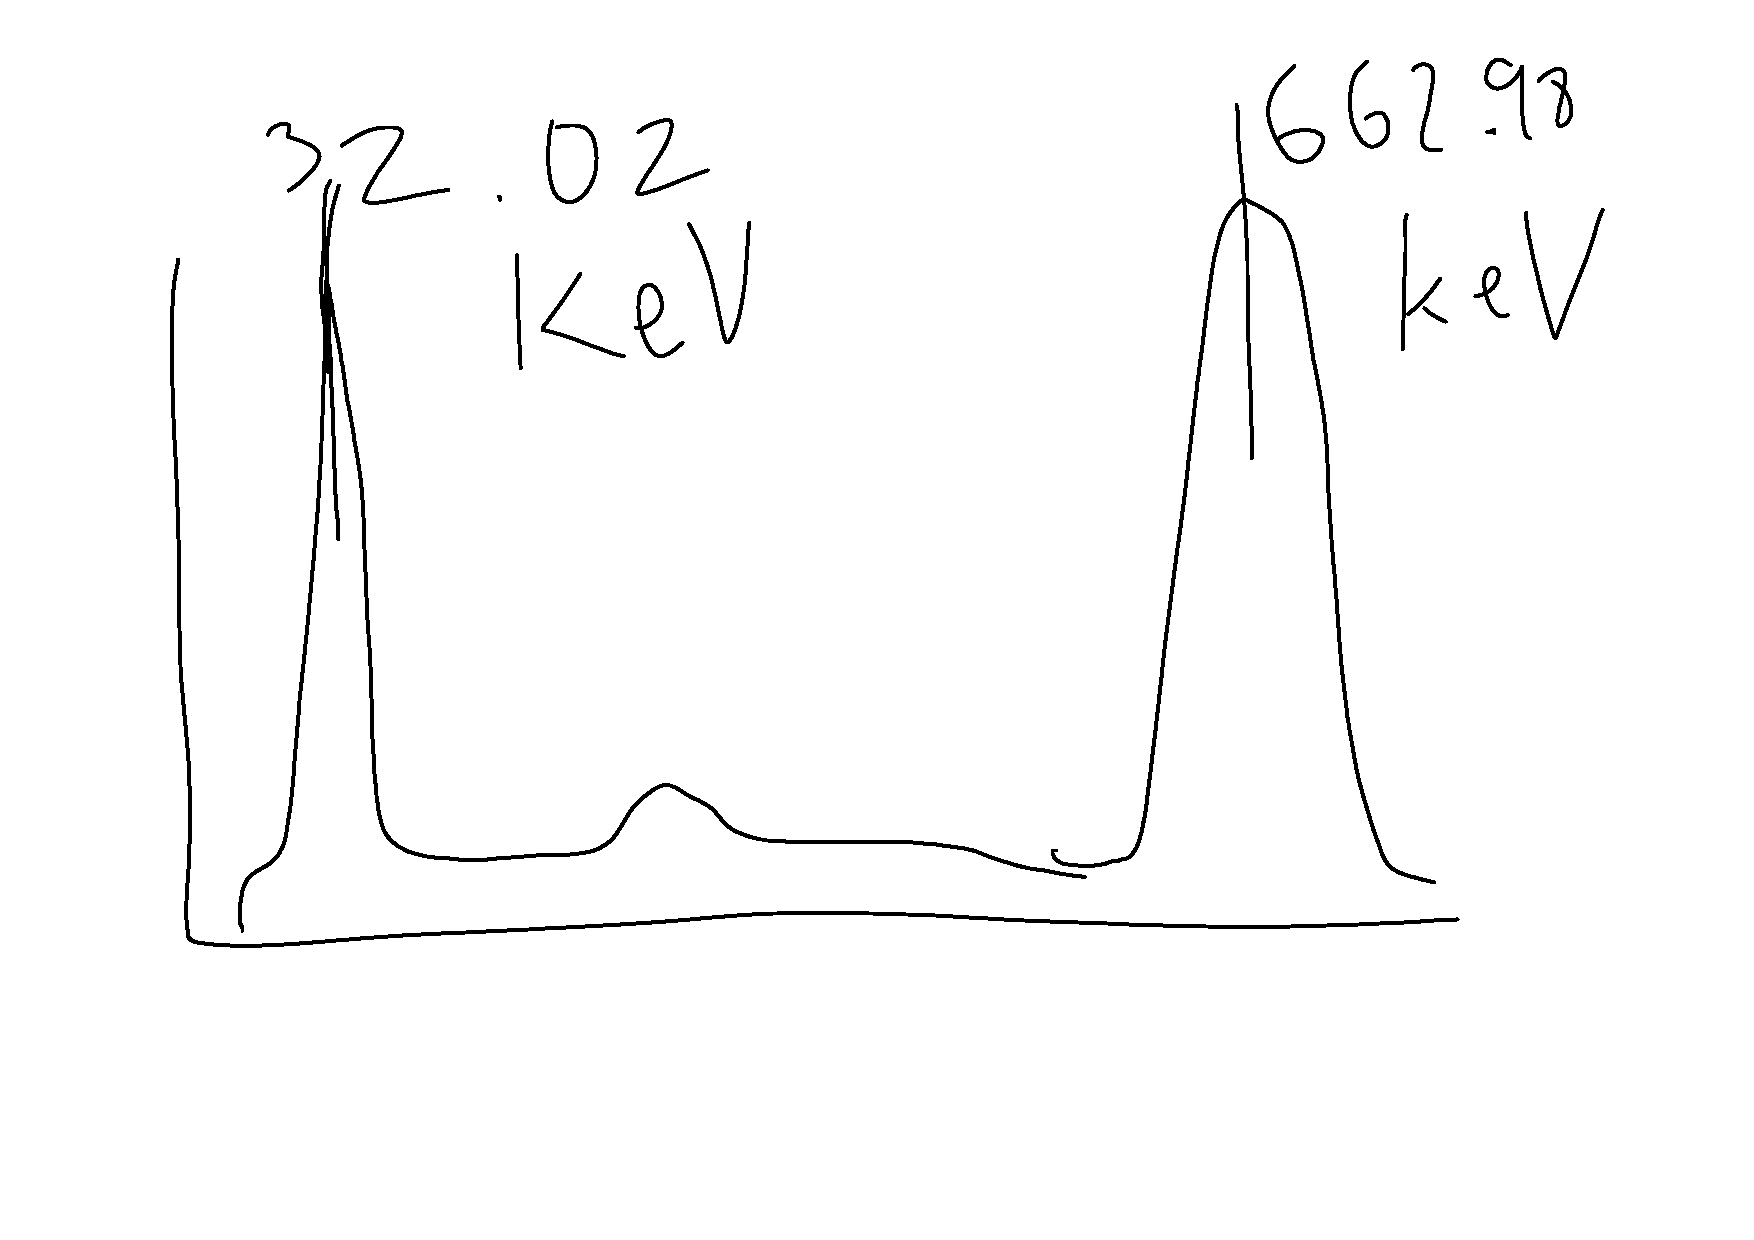
\includegraphics[width=0.75\textwidth]{figures/cesium_137_counts.pdf}
    \caption{$^{137}$Cspectra of counts associated with varying energy bins. Two distinct peaks were identified, with the photo electric peak being centered (after calibration) at 662.98 keV, and the secondary peak presenting at 32.02 keV. A backscatter peak was recorded roughly between the two, however was not measured.}title
\end{figure}
\begin{itemize}
    \item again, cesium was 2.5 cm away from face of detector
    \item 32 keV peak was identified as 32.01 keV, at bin 42.31, with FWHM as 7.21
    \item \verb|$MCA_CAL:-4.452449E+000 8.674188E-001 0.000000E+000 keV|
    \item \textbf{Data saved at: ./data/calibration\_spectrum\_cs.*}
\end{itemize}

\subsection{Spectrum of $^{22}$Na}
\begin{figure}[H]
    \centering
    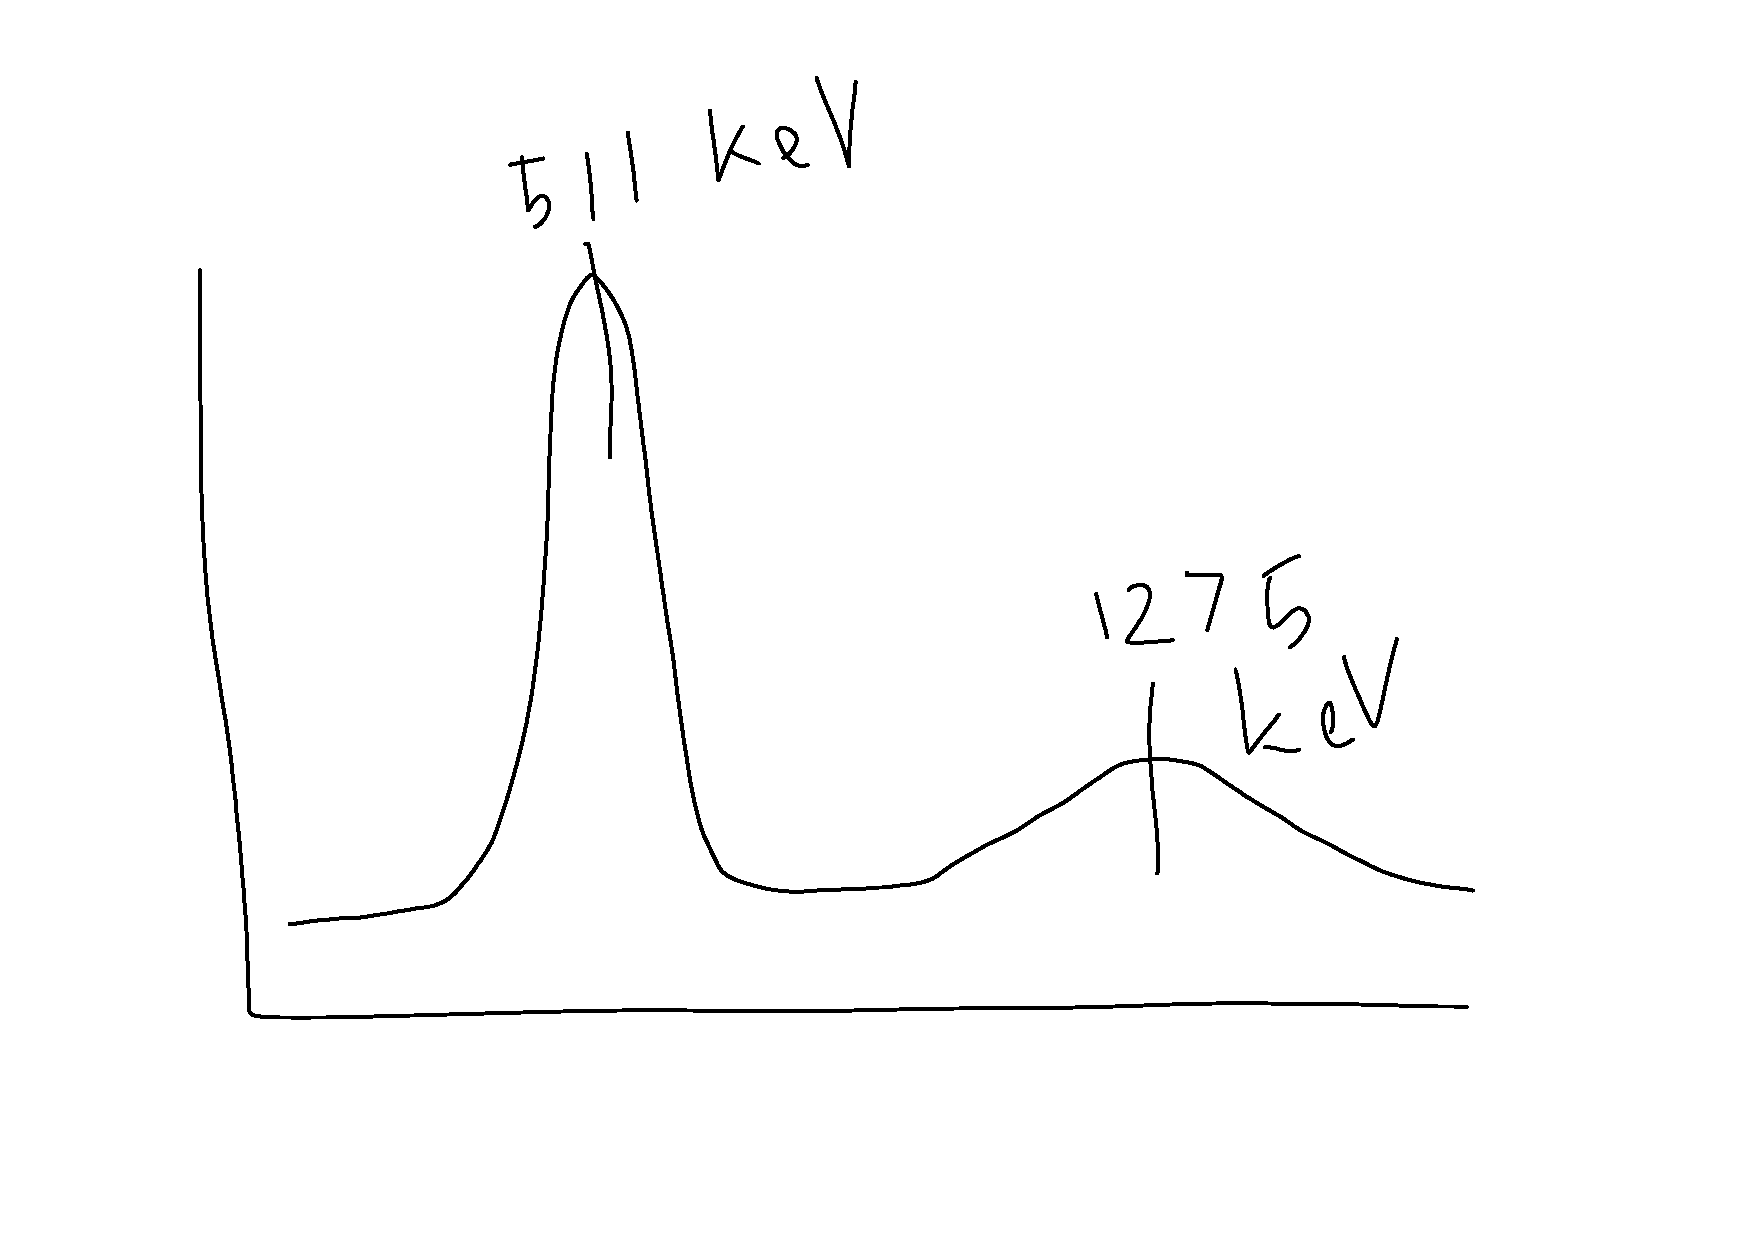
\includegraphics[width=0.75\textwidth]{figures/sodium_22_counts.pdf}
    \caption{$^{22}$Na spectra of counts associated with varying energy bins. Two distinct peaks were identified, with no noticable smaller peaks, the photo electric peak being centered (after calibration) at 1275 keV, and the secondary peak presenting at 511 keV.}
\end{figure}
\begin{itemize}
    \item again, sodium was place 2.5 cm away from face of detector
    \item first uncalibrated peak at 519 keV, bin at 604.34, should be 511 keV, FWHM was 37.65, suggested samarium for 521.28
    \item second uncalibrated peak at 1260.28 keV, at bin 1458.05, should be 1275, FWHM was 57.94
    \item calibration used 1260 peak
    \item after calibration first peak is at 511 keV, FWHM is 38.94, at bin 604.33, library suggests ytrium 88
    \item after calibration second peak is at 1274.54 keV, at bin 1458.04, FWHM was 59.96, library suggests sodium Na-22
    \item \verb|-2.948798E+001 8.943686E-001 0.000000E+000 keV|
    \item \textbf{Data saved at: ./data/calibration\_spectrum\_na.*}
\end{itemize}

\subsection{Spectrum of $^{60}$Co}
\begin{figure}[H]
    \centering
    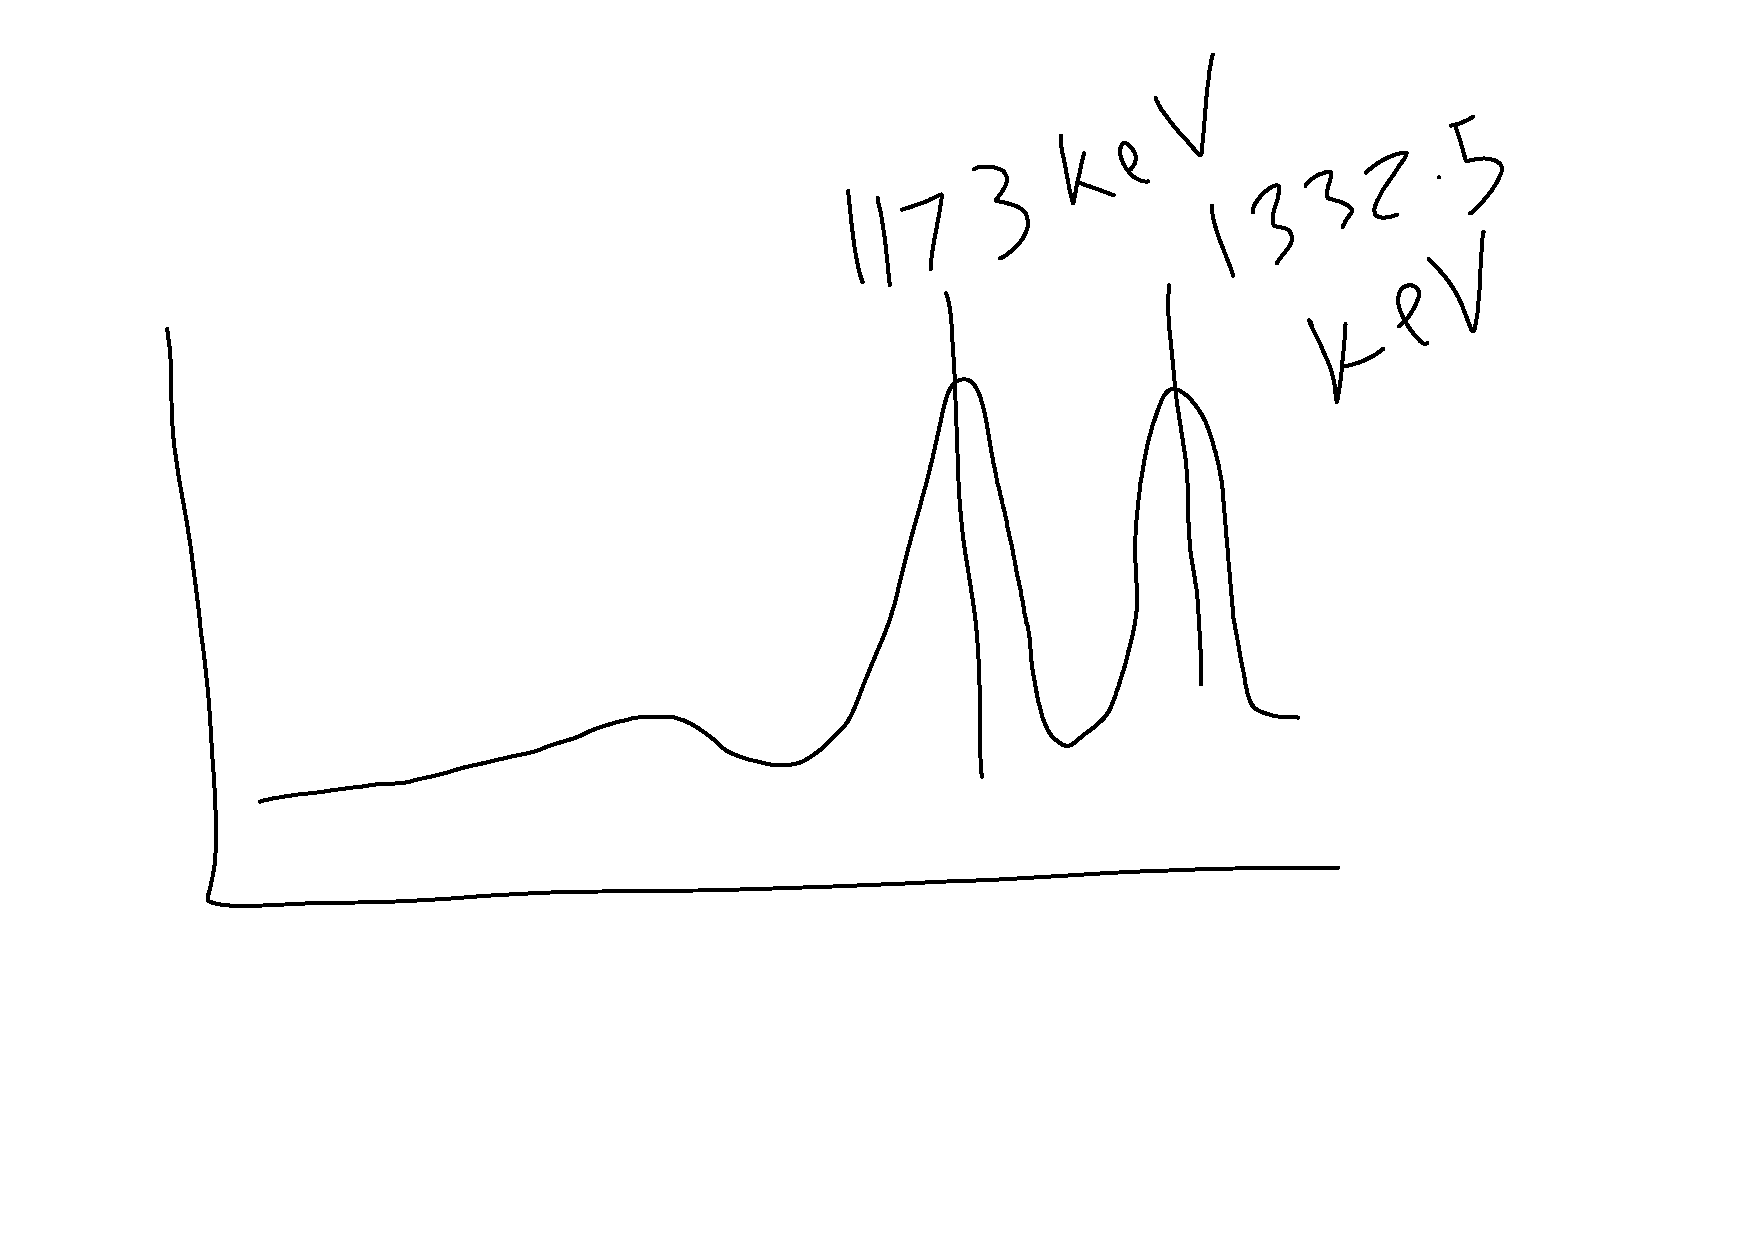
\includegraphics[width=0.75\textwidth]{figures/cobalt_60_counts.pdf}
    \caption{$^{60}$Co spectra of counts associated with varying energy bins. Two distinct peaks were identified, with no noticable smaller peaks, the photo electric peak being centered (after calibration) at 1332.5 keV, and the secondary peak presenting at 1173 keV.}
\end{figure}
\begin{itemize}
    \item again, cobalt was placed 2.5 cm away from face of detector
    \item reading on Oscilloscope was noticably higher than that of cesium and sodium
    \item size of peaks and number of counts on Maestro32 were significantly lower than those of cesium and sodium
    \item two peaks were identified, neighbouring one another
    \item first uncalibrated peak was at 1351 keV, at bin 1544.47, FWHM was 58.80, library suggests Iodine
    \item second uncalibrated peak was at 1192.70 keV, bin was 1366.54, FWHM was 50.96, library suggested Ta-182
    \item first photo peak calibrated to 1173.2 keV (did nothing), second to 1332.5 keV
    \item first peak calibrated to 1173.02 keV, bin at 1366.44, FWHM was 51.17, library suggested cobalt 60
    \item second peak calibrated to 1332.5, at bin 1544.57, FWHM was 64.25, library suggested cobalt 60
    \item \verb|-5.031831E+001 8.952744E-001 0.000000E+000 keV|
    \item \textbf{Data saved at: ./data/calibration\_spectrum\_na.*}
\end{itemize}

\subsection{Background}
\begin{figure}[H]
    \centering
    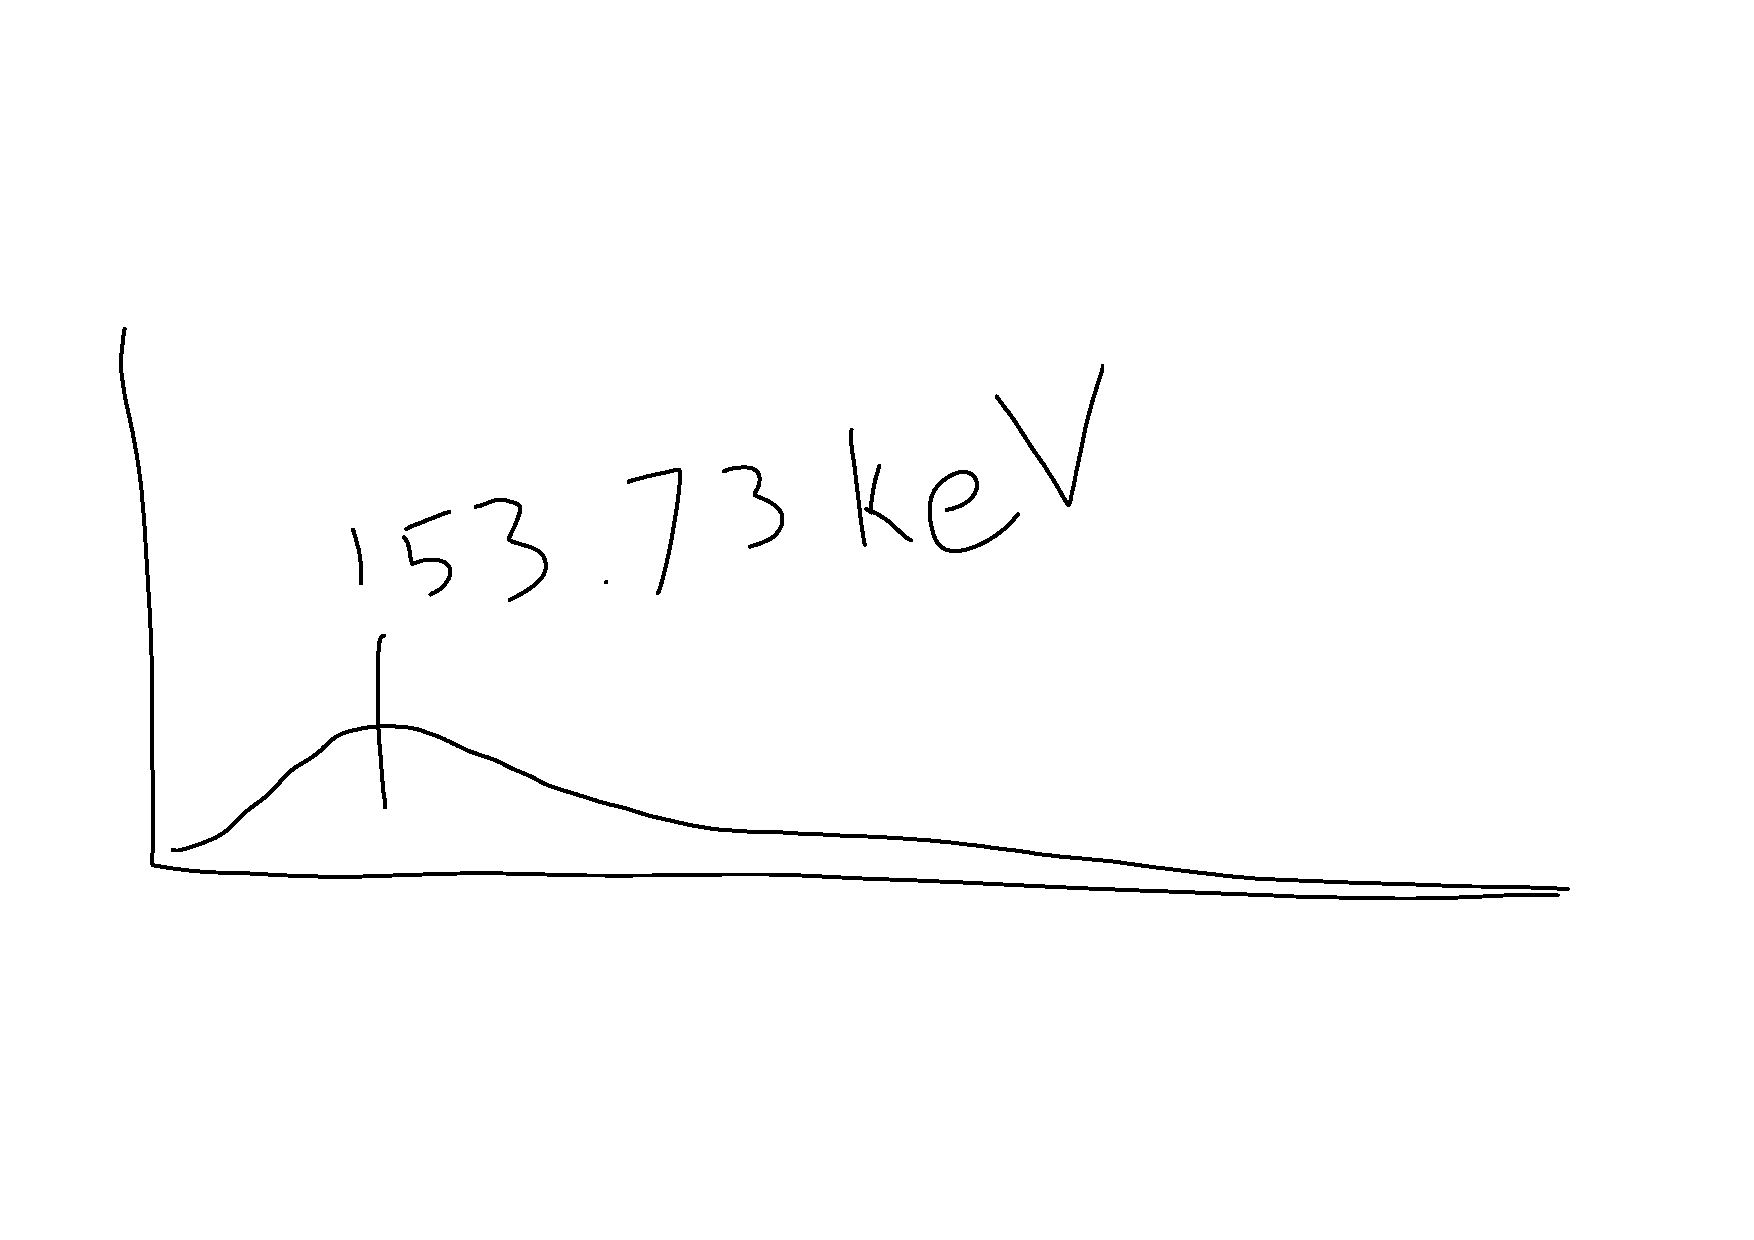
\includegraphics[width=0.75\textwidth]{figures/background_counts.pdf}
    \caption{Background spectra of counts associated with varying energy bins. An elevated count level was identified at 153.73 keV}
\end{figure}
\begin{itemize}
    \item with no sample, a background spectrum was recorded
    \item peak was 153.73 keV, FWHM was 1.04
    \item library suggested xenon 138
    \item \textbf{Data saved at: ./data/calibration\_spectrum\_bg.*}
\end{itemize}

\section{Spectrum and Half-life Measurement of Unknown Sample}

\begin{itemize}
    \item preset time was 60 seconds
    \item Sample was placed 2.5 cm away from source
\end{itemize}
-----------------------------------------------------------
\begin{itemize}
    \item sum of counts was 68493 
    \item recording started at 15:38:19
    \item first peak is at 401.24 keV, peak was at bin 504.38, FWHM was 24.04, library suggests xenon 138
    \item second peak was at 815.92 keV, at bin 967.57, FWHM was 2.20, library suggests lanthanum 140
    \item third peak was at 1096.59 keV, at bin 1281.07, FWHM was 47.07, library suggests iron 59
    \item fourth peak was at 1296.46 keV, FWHM was 44.98, library suggests iodine 132
    \item wait was 5:30 seconds
\end{itemize}
-----------------------------------------------------------
\begin{itemize}
    \item sum of counts was 63755
    \item recording started at 15:45:19
    \item first peak is at 400.52 keV, peak was at bin 503.58, FWHM was 28.25, library suggests selenium 75
    \item second peak was at 799.32 keV, at bin 949.03, FWHM was 22.43, library suggests cs 134
    \item this peak had shifted left a bit
    \item third peak was at 1106.59 keV, at bin 1292.60, FWHM was 17.82, library suggests kr 89
    \item fourth peak was at 1295.25 keV, FWHM was 48.99, library suggests iodine 132, bin 1502.96
    \item wait was 5:30 seconds
\end{itemize}
-----------------------------------------------------------
\begin{itemize}
    \item sum of counts was 59850
    \item recording started at 15:51:58
    \item first peak is at 401.25 keV, peak was at bin 504.40, FWHM was 26.44, library suggests xenon 138
    \item second peak was at 796.80 keV, at bin 946.21, FWHM was 1.04, library suggests cs 134 (this peak had almost disappeared)
    \item third peak was at 1099.32 keV, at bin 1284.12, FWHM was 27.57, library suggests iron 59
    \item fourth peak was at 1293.16 keV, FWHM was 39.98, library suggests argon 41, bin 1500.64
    \item wait was 5:30 seconds
\end{itemize}
-----------------------------------------------------------
\begin{itemize}
    \item sum of counts was 56863
    \item recording started at 15:58:18
    \item first peak is at 400.35 keV, peak was at bin 503.39, FWHM was 26.55, library suggests selenium 75
    \item second peak was at 759.04 keV, at bin 944.24, FWHM was 15.31, library suggests cs 134 (this peak had almost disappeared)
    \item third peak was at 1097.07 keV, at bin 1281.60, FWHM was 34.67, library suggests iron 59
    \item fourth peak was at 1295.73 keV, FWHM was 42.27, library suggests iodine 134, bin 1503.5
    \item wait was 5:30 seconds
\end{itemize}
-----------------------------------------------------------
\begin{itemize}
    \item sum of counts was 53111
    \item recording started at 16:04:19
    \item first peak is at 401.94 keV, peak was at bin 505.16, FWHM was 26.13, library suggests xenon 138
    \item second peak was at 805.54 keV, at bin 955.95, FWHM was 1.41, library suggests bismuth-214 (this peak has disappeared)
    \item third peak was at 1104.55 keV, at bin 1289.96, FWHM was 10.51, library suggests iodine 135
    \item fourth peak was at 1296.78 keV, FWHM was 38.58, library suggests iodine 133, bin 1504.68
    \item wait was 5:30 seconds
\end{itemize}
-----------------------------------------------------------
\begin{itemize}
    \item sum of counts was 50483
    \item recording started at 16:10:35
    \item first peak is at 400.41 keV, peak was at bin 503.46, FWHM was 21.6, library suggests selenium 75
    \item second peak was at 812.17 keV, at bin 963.38, FWHM was 2.15, library suggests iodine 132 (this peak has disappeared)
    \item third peak was at 1085.92 keV, at bin 1269.15, FWHM was 9.45, library suggests europium 152
    \item fourth peak was at 1292.84 keV, FWHM was 39.26, library suggests argon 41, bin 1500.27
    \item wait was 5:30 seconds
\end{itemize}

\begin{figure}[H]
    \centering
    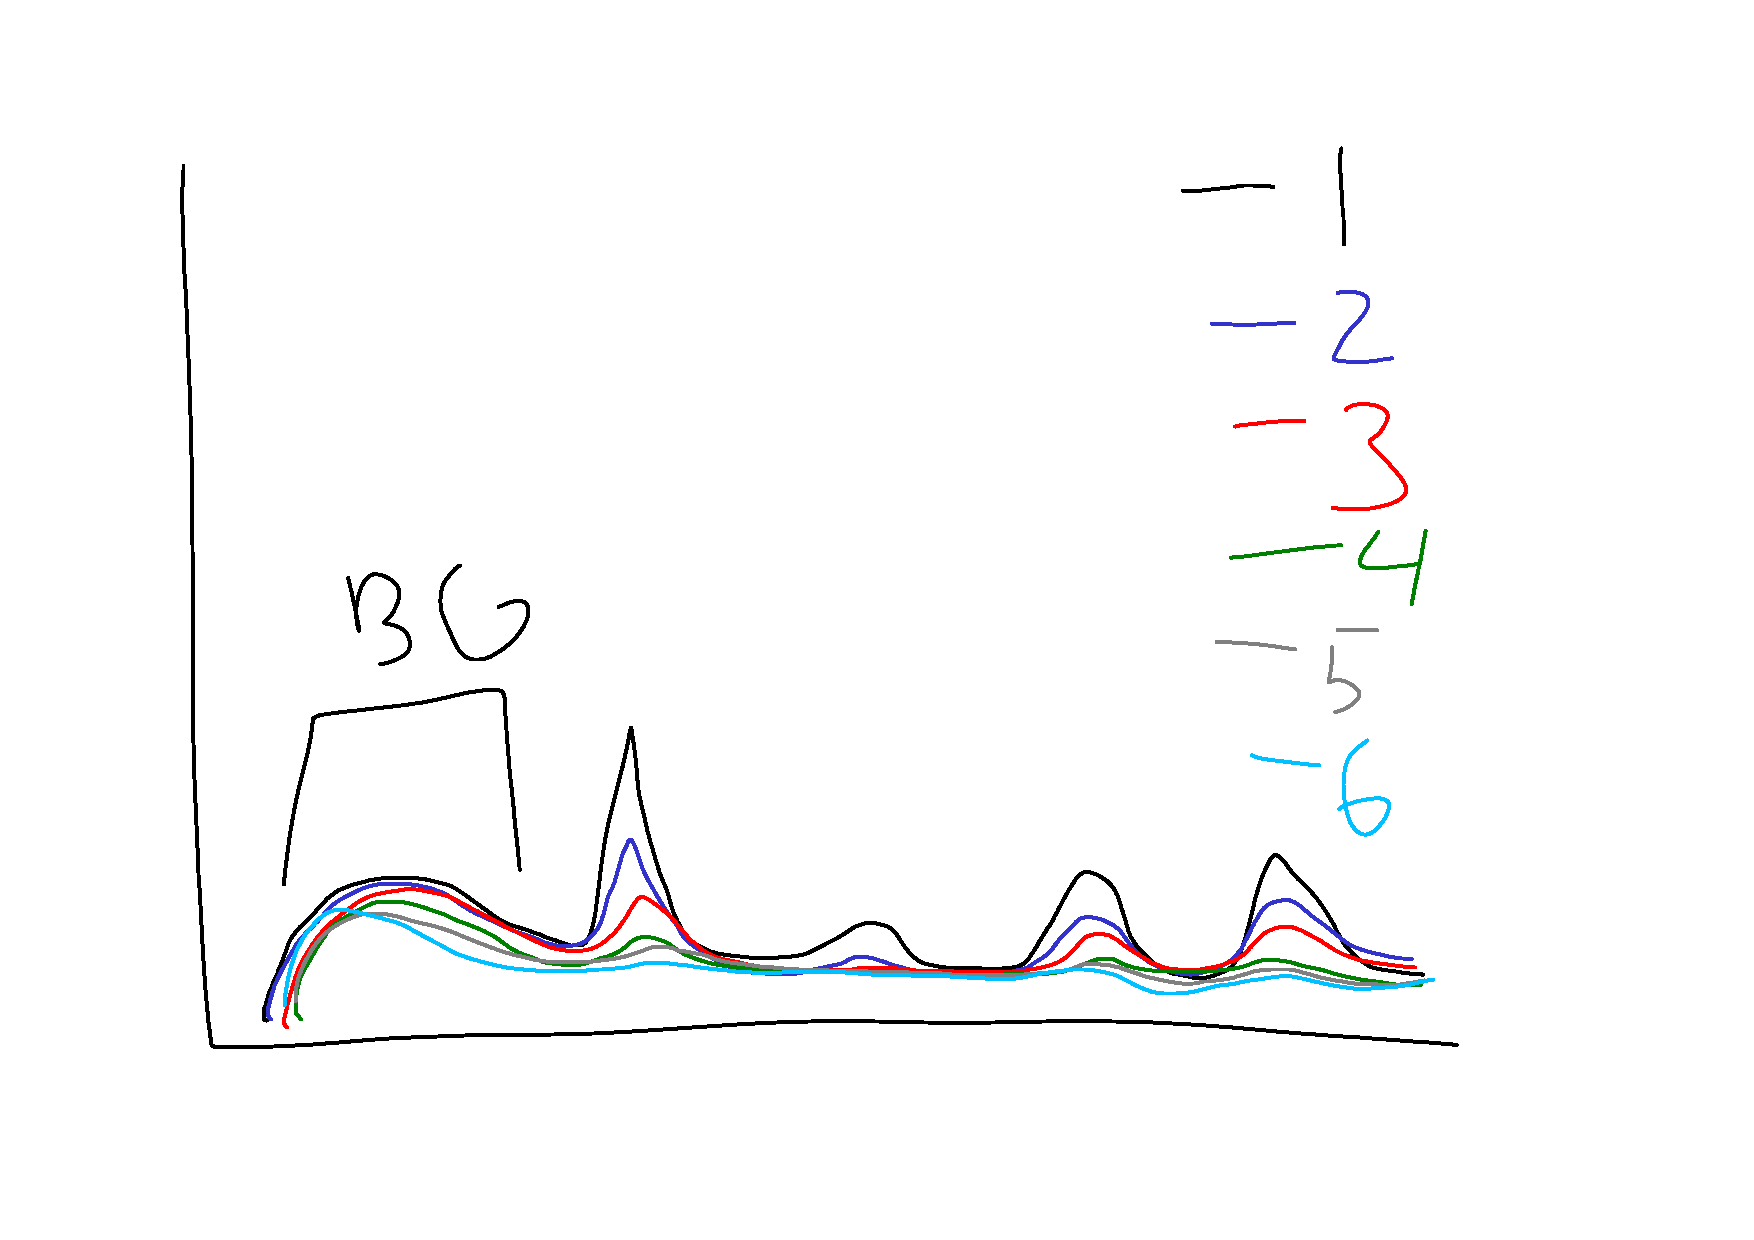
\includegraphics[width=0.75\textwidth]{figures/mystery_isotope.pdf}
    \caption{Spectra of unknown material, with increasing sample number indicating increased sample age. 6 total samples were collected, with 4 primary peaks. Material suggested by software for each peak varied between measurements. The secondary peak disappeared fastest.}
\end{figure}

-----------------------------------------------------------

Data is summarized in~\autoref{tab:counts_v_time}. Based on these values, we suspect that the unknown sample is Indium 116, based on its peaks of 1274 keV and 1085 keV, as well as its half life of 55 minutes. The next candidate was lead, which was ruled out due to its shorter half life, which would have required counts to halve over the course of the experiment. Instead, we observed a 26\% reduction in total counts over the course of approximately 32 minutes or 1936 seconds.
\begin{landscape}

\begin{table}[H]
    \centering
    \caption{Total counts and peak energies with with increasing time since first measurement.}
    \begin{tabular}{c c c c c c c}
        \toprule
        \textbf{Sample Number} & $T+$ & \textbf{Total Counts} & \textbf{Peak 1 Energy} & \textbf{Peak 2 Energy} & \textbf{Peak 3 Energy} & \textbf{Peak 4 Energy} \\
        \midrule
        1 & 0s & 68493 & 401.24 keV &  815.92 keV & 1096.59 keV & 1296.46 keV \\
        2 & 420s & 63755 & 400.52 keV & 799.32 keV & 1106.59 keV & 1295.25 keV \\
        3 & 819s & 59850 & 401.25 keV & 796.80 keV & 1099.32 keV  & 1293.16 keV \\
        4 & 1199s & 56863 & 400.35 keV & 759.04 keV & 1097.07 keV & 1295.73 keV \\
        5 & 1559s & 53111 & 401.94 keV & 805.54 keV & 1104.55 keV & 1296.78 keV \\
        6 & 1936s & 50483 & 400.41 keV & 812.17 keV & 1085.92 keV & 1292.84 keV \\
        \bottomrule
    \end{tabular}
    \label{tab:counts_v_time}
\end{table}

\end{landscape}

\textbf{Data saved at: ./data/mystery\_[1...6].*}

% \begin{equation}
%     I=I_{0}\exp\left(-\lambda t\right)
% \end{equation}

\appendix
% \section{NIM Setup}
\end{document}